\begin{frame}[t]{\secname}{\subsecname{} - Why \& Implementation}

\begin{itemize}
  \item Ensure effect causing failure adequately described \& robust solution
  %\item Check solution dependency on underlying discretization scheme
  \item Prove influence on damage of
  \begin{itemize}[noitemsep]
    \item Scatter in stress-strain-curves, micro-voids \& findings in micrographs
    \item Varying degree of cure, disparities from machining
  \end{itemize}
\end{itemize}

\setlength{\figheight}{0.475\textheight}
\begin{columns}[t]
  \begin{column}{0.5\textwidth}
    \only<2->{
      \begin{block}{Stochastic model}
        \centering
        % Variables
        \def\nb{20}
        \def\ne{10}
        % Picture
        \tikzexternalenable
        \tikzsetnextfilename{Implementation_Stochastic_Constant}
        \begin{tikzpicture}
  \begin{axis}[
    width=\linewidth,
    height=\figheight,
    ybar,
    bar shift=0pt,
    %axis lines=middle,
    axis x line=bottom,
    axis y line=middle,
    samples=10,
    enlarge y limits=upper,
    xmin=-\ne/2-0.75,
    xmax= \ne/2+0.75,
    ymin=0,
    ymax=(\nb+1)*1.05,
    xlabel=$K$,
    ylabel=$n_e$,
    x label style={at={(axis description cs:1.0,0.0)},anchor=south west},
    y label style={at={(axis description cs:0.5,1.0)},anchor=south west},
    %xtick={-\ne/2,0,\ne/2},
    xtick={-5,0,5},
    ymajorticks=false,
    xticklabels={$\bar{K}-\Delta$,$\bar{K}$,$\bar{K}+\Delta$},
    yticklabels={},
  ]
    %\addplot +[black,fill=gray]{rnd};
    %\addplot coordinates {(-\ne/2,\nb)};
    \foreach \x in {-5,-4,...,5} {
      \addplot+[black,fill=gray] coordinates {(\x,\nb+rand)};%,bar shift=0.5
    }
  \end{axis}
\end{tikzpicture}
        \tikzexternaldisable
      \end{block}
    }
  \end{column}
  \begin{column}{0.5\textwidth}
    \only<3->{
      \begin{block}{Base FE model}
        \centering
        \includegraphics[width=0.85\linewidth,height=\figheight,keepaspectratio]{Model_FE_Hex_0-5_Stochastic_ct}
      \end{block}
    }
  \end{column}
\end{columns}
  
\end{frame}


% \begin{figure}[htbp]
%   \setlength{\figheight}{5cm}
%   \begin{subfigure}{0.49\linewidth}
%     \begin{minipage}[b][\figheight]{\linewidth}
%       \centering
%       % Variables
%       \def\nb{20}
%       \def\ne{10}
%       % Picture
%       \begin{tikzpicture}
  \begin{axis}[
    width=\linewidth,
    height=\figheight,
    ybar,
    bar shift=0pt,
    %axis lines=middle,
    axis x line=bottom,
    axis y line=middle,
    samples=10,
    enlarge y limits=upper,
    xmin=-\ne/2-0.75,
    xmax= \ne/2+0.75,
    ymin=0,
    ymax=(\nb+1)*1.05,
    xlabel=$K$,
    ylabel=$n_e$,
    x label style={at={(axis description cs:1.0,0.0)},anchor=south west},
    y label style={at={(axis description cs:0.5,1.0)},anchor=south west},
    %xtick={-\ne/2,0,\ne/2},
    xtick={-5,0,5},
    ymajorticks=false,
    xticklabels={$\bar{K}-\Delta$,$\bar{K}$,$\bar{K}+\Delta$},
    yticklabels={},
  ]
    %\addplot +[black,fill=gray]{rnd};
    %\addplot coordinates {(-\ne/2,\nb)};
    \foreach \x in {-5,-4,...,5} {
      \addplot+[black,fill=gray] coordinates {(\x,\nb+rand)};%,bar shift=0.5
    }
  \end{axis}
\end{tikzpicture}
%     \end{minipage}
%     \caption{Simple stochastic model}
%     \label{fig:Thry:Stochastic:Distribution}
%   \end{subfigure}
%   \hfill
%   \begin{subfigure}{0.49\linewidth}
%     \begin{minipage}[b][\figheight]{\linewidth}
%       %\includegraphics[width=\linewidth,height=\figheight,keepaspectratio]{../../Material/Figures/Model_FE_Hex_0-5_Stochastic_ct.png}
%       \includegraphics[width=\linewidth,height=\figheight,keepaspectratio]{Model_FE_Hex_0-5_Stochastic_ct}
%     \end{minipage}
%     \caption{Base FE mesh with stochastic block distribution}
%     \label{fig:Thry:Stochastic:FEModel}
%   \end{subfigure}
%   \caption{Implementation of stochastic material distribution for PD simulations}
%   \label{fig:Thry:Stochastic:Implementation}
% \end{figure}